\documentclass[12pt, letterpaper]{article}

\usepackage{color} %% Allows text to be typeset in color.

%% These allow Me to add Images to the Book.
\usepackage{graphicx}
\graphicspath{ {images/} }

%% Enables hyperlinks.
\usepackage{hyperref}

%% Makes BigO easier.
\newcommand{\bigO}{\mathcal{O}}
\newcommand{\bigOmega}{\Omega}
\newcommand{\bigTheta}{\Theta}

%%
\oddsidemargin0cm
\evensidemargin0cm
\topmargin-2cm     % These lines increase the amount of usable space and save trees.
\textwidth16.5cm
\textheight23.5cm  

%%\setcounter{tocdepth}{4} %% set the table of contents detail depth.

%% Types of organizational sections.s
%%\part{}
%%\chapter{}
%%\section{}
%%\subsection{}
%%\subsubsection{}
%%\paragraph{}
%%\subparagraph{}

\begin{document}

\title{\color{blue}Hump Yard Rules v1.3}
\author{Written by Bryce Summers \texttt(BryceSummers.com)}
\date{\color{red}Last Updated: \today}
\maketitle

\tableofcontents 

\section{Overview}

Hump Yard is a game about creating the most efficient yard possible in order to win more sorting contracts than your opponents.

\newpage
\section{Components}

Hump Yard comes with 4 of each of the following \textit{normal} Track tiles:


\includegraphics[width=0.20\textwidth]{Track_0.png}

\includegraphics[width=0.20\textwidth]{Track_3.png}
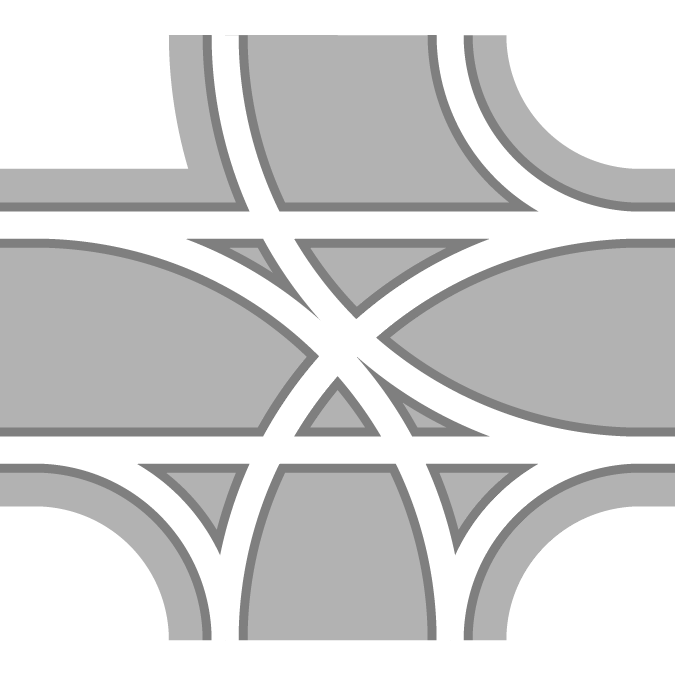
\includegraphics[width=0.20\textwidth]{Track_10.png}

\includegraphics[width=0.20\textwidth]{Track_22.png}

\includegraphics[width=0.20\textwidth]{Track_25.png}
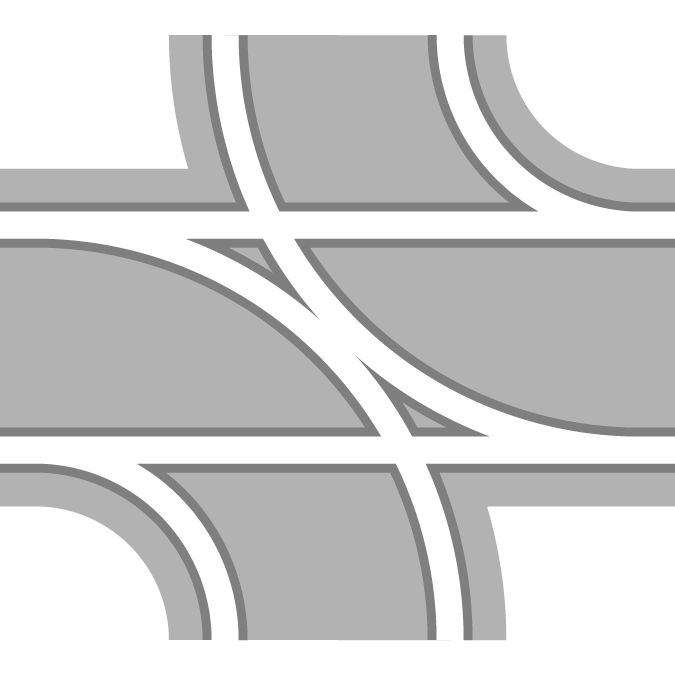
\includegraphics[width=0.20\textwidth]{Track_26.png}

\includegraphics[width=0.20\textwidth]{Track_32.png}

\includegraphics[width=0.20\textwidth]{Track_35.png}
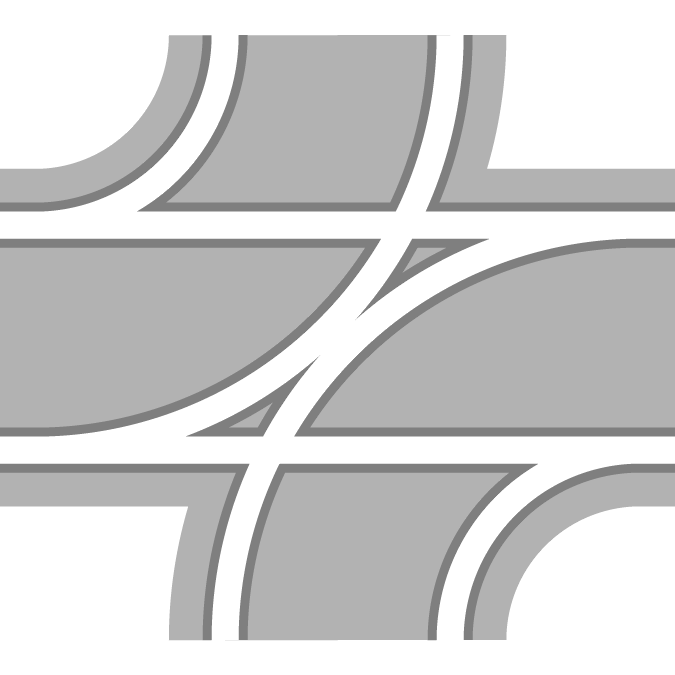
\includegraphics[width=0.20\textwidth]{Track_38.png}

\includegraphics[width=0.20\textwidth]{Track_39.png}

\includegraphics[width=0.20\textwidth]{Track_40.png}

\includegraphics[width=0.20\textwidth]{Track_41.png}

\includegraphics[width=0.20\textwidth]{Track_43.png}

\includegraphics[width=0.20\textwidth]{Track_44.png}

\includegraphics[width=0.20\textwidth]{Track_45.png}

\includegraphics[width=0.20\textwidth]{Track_55.png}

\includegraphics[width=0.20\textwidth]{Track_57.png}
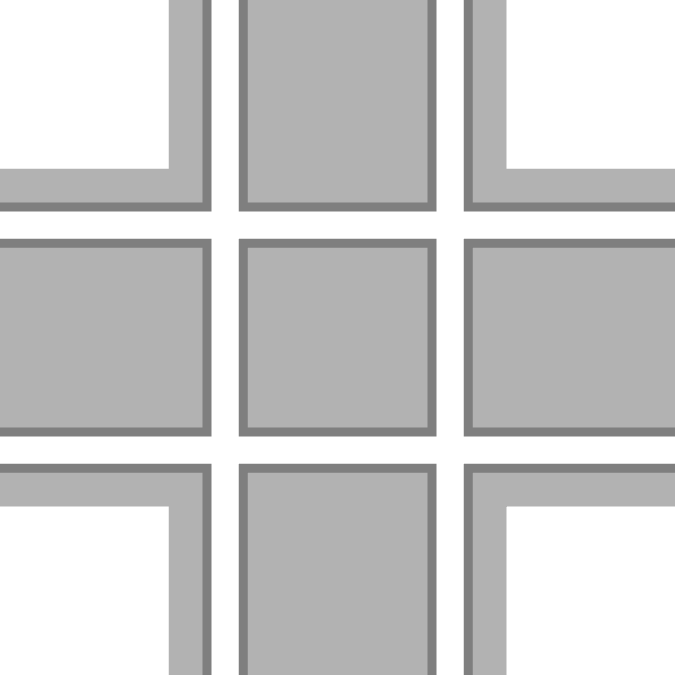
\includegraphics[width=0.20\textwidth]{Track_60.png}
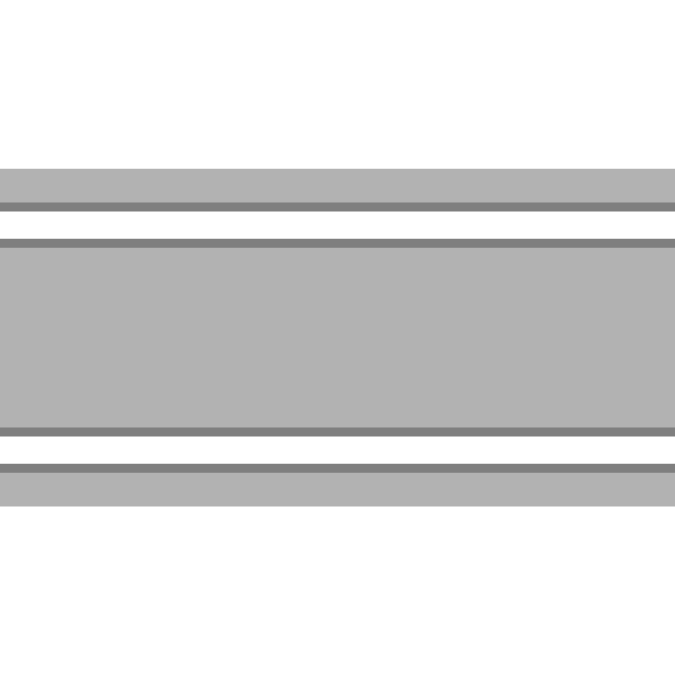
\includegraphics[width=0.20\textwidth]{Track_62.png}
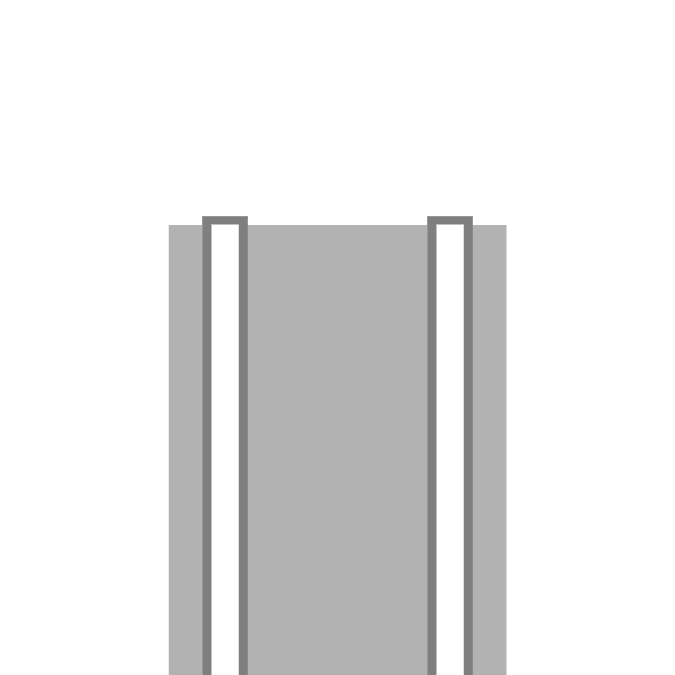
\includegraphics[width=0.20\textwidth]{Track_end.png}

5 of each of the following colored track headings:

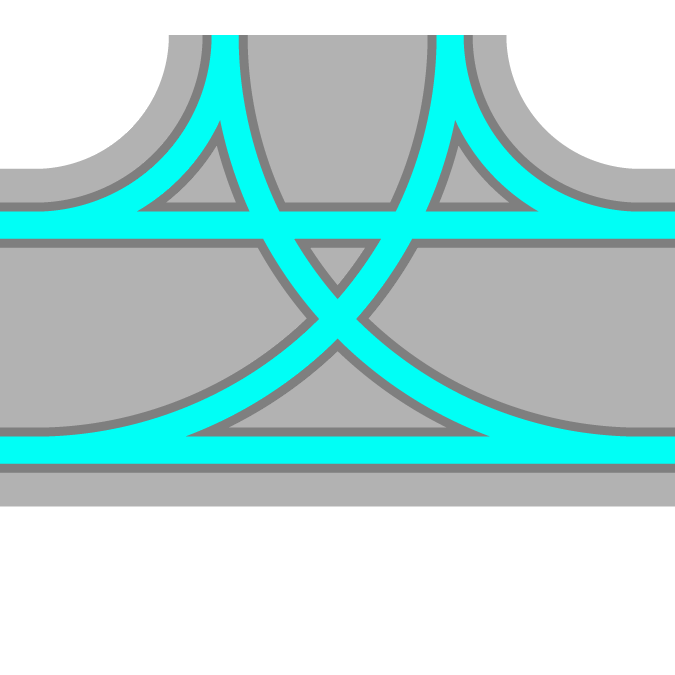
\includegraphics[width=0.20\textwidth]{BlueHeading.png}
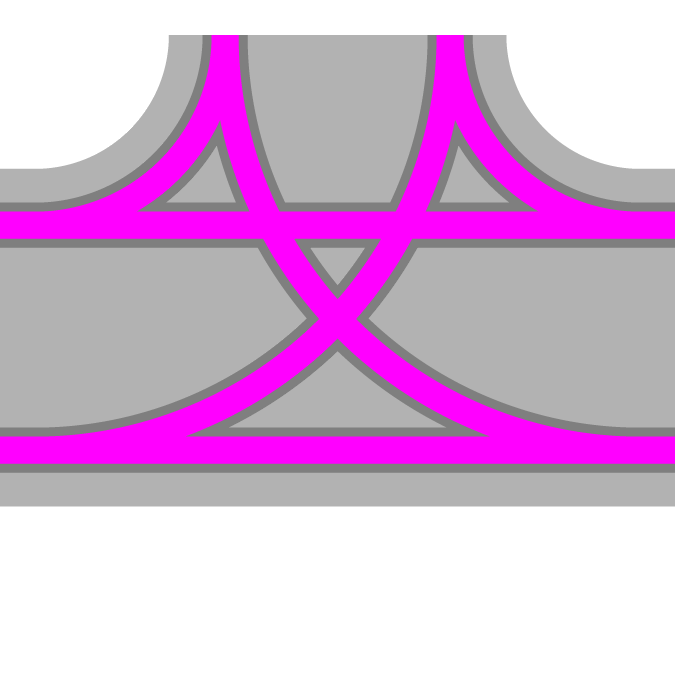
\includegraphics[width=0.20\textwidth]{PurpleHeading.png}
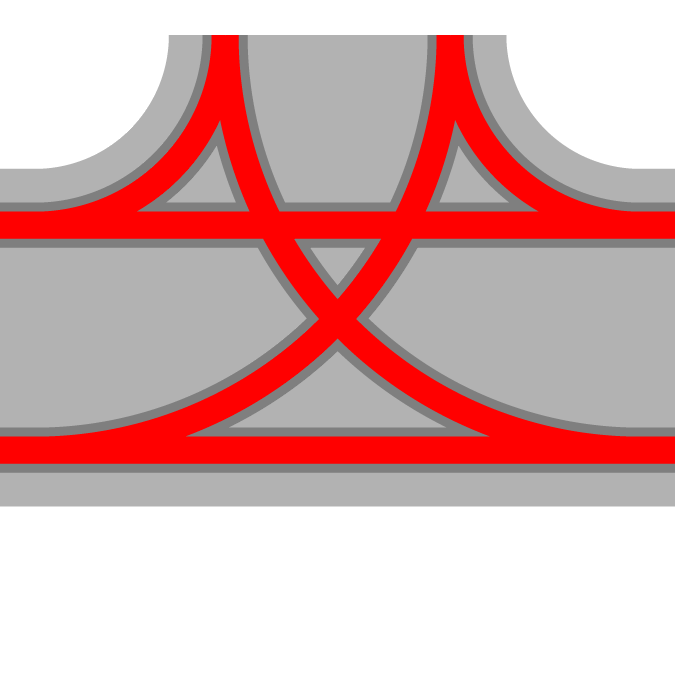
\includegraphics[width=0.20\textwidth]{RedHeading.png}
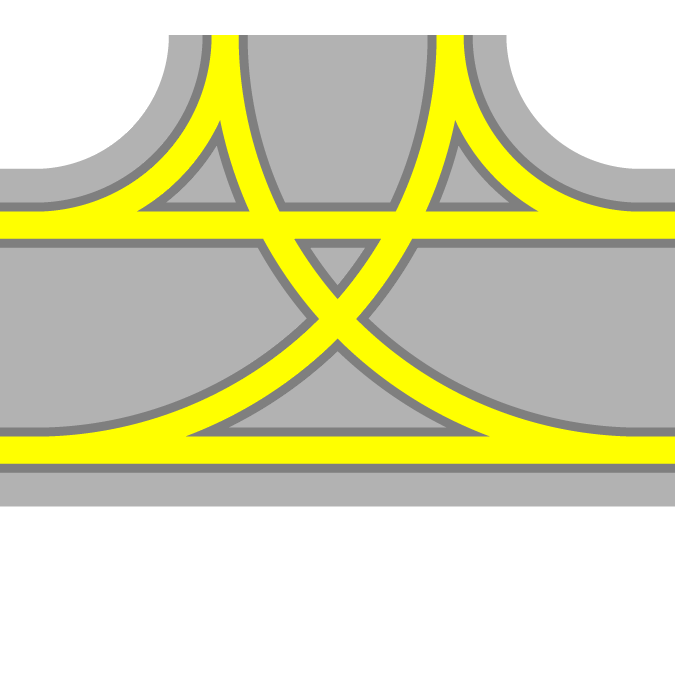
\includegraphics[width=0.20\textwidth]{YellowHeading.png}

8 Sources and 8 Sinks.

\includegraphics[width=0.25\textwidth]{Source.png} $\times 8$

\includegraphics[width=0.25\textwidth]{Sink.png} $\times 8$

Pieces, Colorful Car cards.


\section{Rules of Play}

\subsection{Setup}

Every players sets up their yard as follows with 5 of their collored heading tracks sandwitched by a source and a sink:


\includegraphics[width=0.10\textwidth]{Source.png}
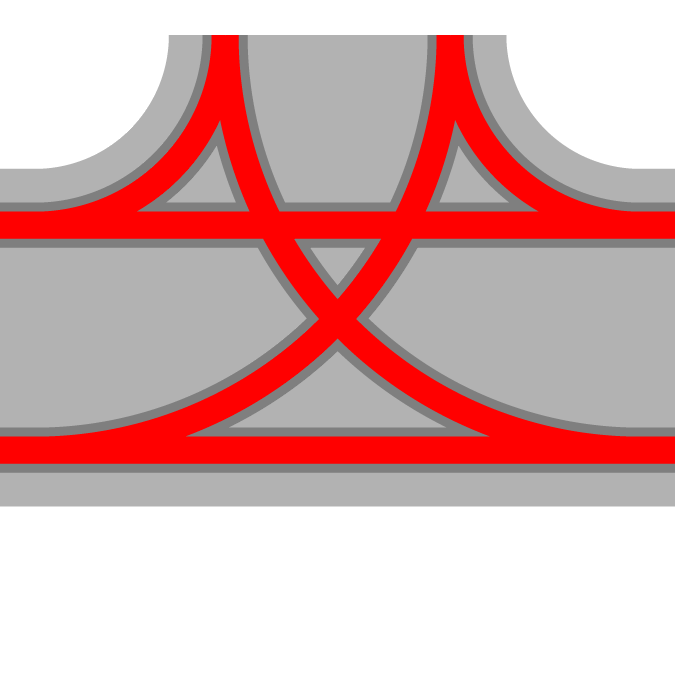
\includegraphics[width=0.10\textwidth]{RedHeading.png}
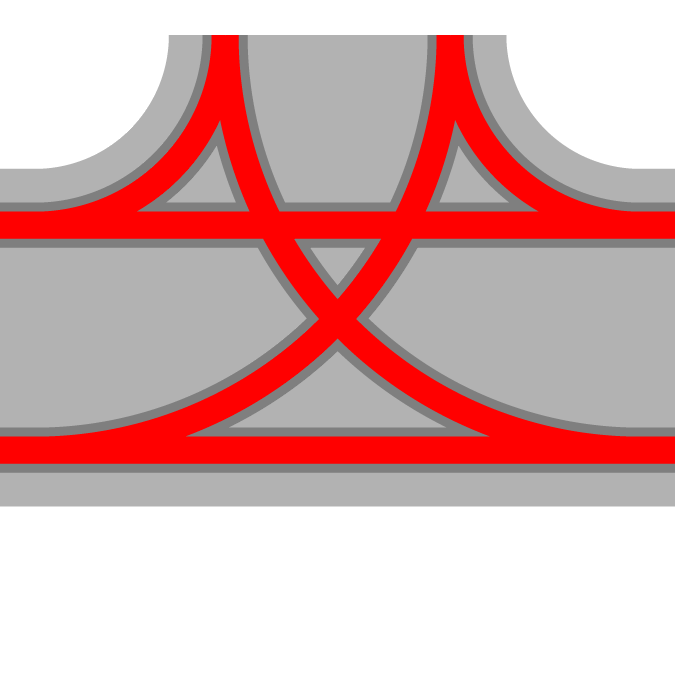
\includegraphics[width=0.10\textwidth]{RedHeading.png}
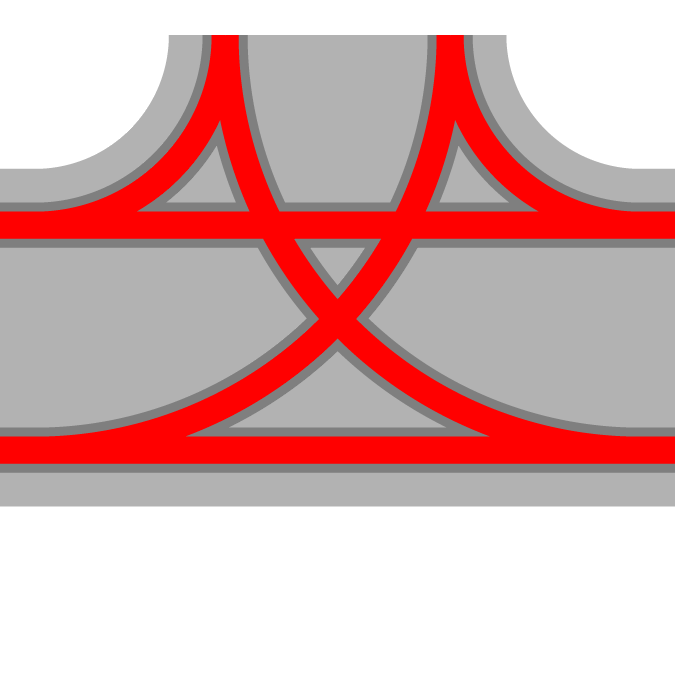
\includegraphics[width=0.10\textwidth]{RedHeading.png}
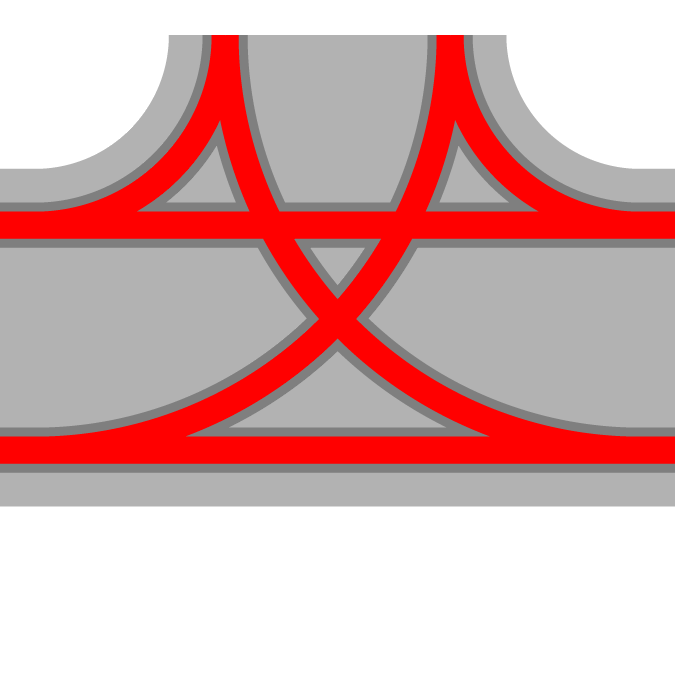
\includegraphics[width=0.10\textwidth]{RedHeading.png}
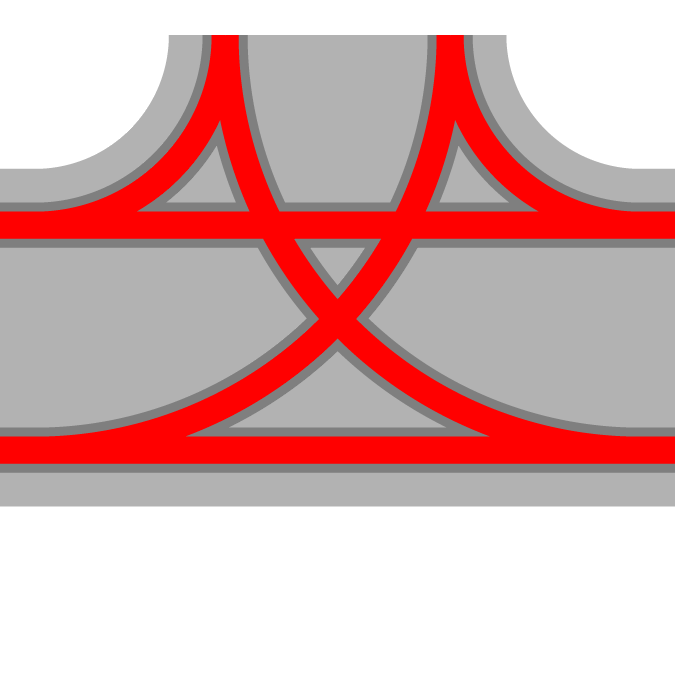
\includegraphics[width=0.10\textwidth]{RedHeading.png}

\includegraphics[width=0.10\textwidth]{Sink.png}

It is perfectly fine to have the headings point downwards if desired.

Place all of the track tiles in a stack face down.

Choose a player to be the start player.

Players start the game with 0 points.

\subsection{Turns}

Each turn consists of the following phases.

\subsubsection{Phase 1 : New Track}

Reveal 1 track piece per player and set them in the middle of the table.

In order from the player with the least points to the player with the most points, players choose 1 piece of track and build it next to a tile in their yard.

In the case of a tie in the number of points, the tie is broken in clock - wise order from the start player.

Track pieces in a yard must all be connected horizontally or vertically.

\subsubsection{Phase 2 : Bidding on a Train sorting contract.}

Reveal 2 car cards and set them out in order in the middle of the table.

Players bid on the number of moves they think they could use to proccess the train after the order of the cars has been randomly shuffled.

Players may also request that an additional number of cars may be revealed from the deck and appended to the end of train and make a bid on the number of moves it would take them to properly shuffle the longer train.

\subsubsection{Phase 3 : Determining the winner of the train.}

Every player takes car pieces identical to the sub train that they bid on and line them up in order at the source of their yard.

The revealed set of car cards is shuffled together and then a permutation of the original train is revealed. If the lowest bidder for that length of train can successfully sort the original train into the generated permutation using no more than the number of moves that they bid, then they win all of the car cards.

If nobody was able to fullfill their bid, then the proccess is repeated with the cars consisting of the next smaller sub train that was bid on.

If nobody fullfills their bid, then the cars are sent to a discard pile.

Players keep their won car cards and these count as the player's points.

\subsubsection{Phase 4: End of Turn.}

The player with the fewest points receives the start player token. In the event of a tie, the person with the fewest points and closest clockwise from the previous start player is chosen. (In other words the start player is gurranteed to change in the event of a tie.)

\subsection{Legal Moves}

A set of connected cars may be moved as far as possible in one direction. Cars may be interpretted as coupled or uncoupled at the beginning of the move, but the interpretation cannot be changed until the next moves, in other words if you wish to move and connect cars, you will have to move the first train to the other train, then end the move. During your next move, you may interpret the cars as coupled into one train.

To properly exit a train from the yard, every car must be coupled and be in the order specified by the random permuation.

\subsection{End of Game and Winning}

The game ends after 20 turns or when the car card deck is exhausted.

The player wth the most number of car cards wins the game.

%% Signals that the document has ended.
\end{document}